\documentclass[twoside]{book}

% Packages required by doxygen
\usepackage{fixltx2e}
\usepackage{calc}
\usepackage{doxygen}
\usepackage[export]{adjustbox} % also loads graphicx
\usepackage{graphicx}
\usepackage[utf8]{inputenc}
\usepackage{makeidx}
\usepackage{multicol}
\usepackage{multirow}
\PassOptionsToPackage{warn}{textcomp}
\usepackage{textcomp}
\usepackage[nointegrals]{wasysym}
\usepackage[table]{xcolor}

% Font selection
\usepackage[T1]{fontenc}
\usepackage[scaled=.90]{helvet}
\usepackage{courier}
\usepackage{amssymb}
\usepackage{sectsty}
\renewcommand{\familydefault}{\sfdefault}
\allsectionsfont{%
  \fontseries{bc}\selectfont%
  \color{darkgray}%
}
\renewcommand{\DoxyLabelFont}{%
  \fontseries{bc}\selectfont%
  \color{darkgray}%
}
\newcommand{\+}{\discretionary{\mbox{\scriptsize$\hookleftarrow$}}{}{}}

% Page & text layout
\usepackage{geometry}
\geometry{%
  a4paper,%
  top=2.5cm,%
  bottom=2.5cm,%
  left=2.5cm,%
  right=2.5cm%
}
\tolerance=750
\hfuzz=15pt
\hbadness=750
\setlength{\emergencystretch}{15pt}
\setlength{\parindent}{0cm}
\setlength{\parskip}{3ex plus 2ex minus 2ex}
\makeatletter
\renewcommand{\paragraph}{%
  \@startsection{paragraph}{4}{0ex}{-1.0ex}{1.0ex}{%
    \normalfont\normalsize\bfseries\SS@parafont%
  }%
}
\renewcommand{\subparagraph}{%
  \@startsection{subparagraph}{5}{0ex}{-1.0ex}{1.0ex}{%
    \normalfont\normalsize\bfseries\SS@subparafont%
  }%
}
\makeatother

% Headers & footers
\usepackage{fancyhdr}
\pagestyle{fancyplain}
\fancyhead[LE]{\fancyplain{}{\bfseries\thepage}}
\fancyhead[CE]{\fancyplain{}{}}
\fancyhead[RE]{\fancyplain{}{\bfseries\leftmark}}
\fancyhead[LO]{\fancyplain{}{\bfseries\rightmark}}
\fancyhead[CO]{\fancyplain{}{}}
\fancyhead[RO]{\fancyplain{}{\bfseries\thepage}}
\fancyfoot[LE]{\fancyplain{}{}}
\fancyfoot[CE]{\fancyplain{}{}}
\fancyfoot[RE]{\fancyplain{}{\bfseries\scriptsize Generated by Doxygen }}
\fancyfoot[LO]{\fancyplain{}{\bfseries\scriptsize Generated by Doxygen }}
\fancyfoot[CO]{\fancyplain{}{}}
\fancyfoot[RO]{\fancyplain{}{}}
\renewcommand{\footrulewidth}{0.4pt}
\renewcommand{\chaptermark}[1]{%
  \markboth{#1}{}%
}
\renewcommand{\sectionmark}[1]{%
  \markright{\thesection\ #1}%
}

% Indices & bibliography
\usepackage{natbib}
\usepackage[titles]{tocloft}
\setcounter{tocdepth}{3}
\setcounter{secnumdepth}{5}
\makeindex

% Hyperlinks (required, but should be loaded last)
\usepackage{ifpdf}
\ifpdf
  \usepackage[pdftex,pagebackref=true]{hyperref}
\else
  \usepackage[ps2pdf,pagebackref=true]{hyperref}
\fi
\hypersetup{%
  colorlinks=true,%
  linkcolor=blue,%
  citecolor=blue,%
  unicode%
}

% Custom commands
\newcommand{\clearemptydoublepage}{%
  \newpage{\pagestyle{empty}\cleardoublepage}%
}

\usepackage{caption}
\captionsetup{labelsep=space,justification=centering,font={bf},singlelinecheck=off,skip=4pt,position=top}

%===== C O N T E N T S =====

\begin{document}

% Titlepage & ToC
\hypersetup{pageanchor=false,
             bookmarksnumbered=true,
             pdfencoding=unicode
            }
\pagenumbering{alph}
\begin{titlepage}
\vspace*{7cm}
\begin{center}%
{\Large Proyecto\+\_\+\+Segmentacion\+\_\+\+Temporal \\[1ex]\large 0.\+1.\+0 }\\
\vspace*{1cm}
{\large Generated by Doxygen 1.8.12}\\
\end{center}
\end{titlepage}
\clearemptydoublepage
\pagenumbering{roman}
\tableofcontents
\clearemptydoublepage
\pagenumbering{arabic}
\hypersetup{pageanchor=true}

%--- Begin generated contents ---
\chapter{Namespace Index}
\section{Packages}
Here are the packages with brief descriptions (if available)\+:\begin{DoxyCompactList}
\item\contentsline{section}{\hyperlink{namespacemainengine}{mainengine} }{\pageref{namespacemainengine}}{}
\item\contentsline{section}{\hyperlink{namespaceserver}{server} }{\pageref{namespaceserver}}{}
\item\contentsline{section}{\hyperlink{namespaceunittests}{unittests} }{\pageref{namespaceunittests}}{}
\end{DoxyCompactList}

\chapter{Hierarchical Index}
\section{Class Hierarchy}
This inheritance list is sorted roughly, but not completely, alphabetically\+:\begin{DoxyCompactList}
\item \contentsline{section}{mainengine.\+Distance\+Histogram\+Generator}{\pageref{interfacemainengine_1_1_distance_histogram_generator}}{}
\begin{DoxyCompactList}
\item \contentsline{section}{mainengine.\+Bhattacharyya\+Handler}{\pageref{classmainengine_1_1_bhattacharyya_handler}}{}
\end{DoxyCompactList}
\item \contentsline{section}{mainengine.\+Histogram\+Processor}{\pageref{classmainengine_1_1_histogram_processor}}{}
\item \contentsline{section}{mainengine.\+Main\+Processor}{\pageref{classmainengine_1_1_main_processor}}{}
\item \contentsline{section}{server.\+My\+Web\+Socket\+Handler}{\pageref{classserver_1_1_my_web_socket_handler}}{}
\item \contentsline{section}{mainengine.\+Stadistical\+Calculator}{\pageref{interfacemainengine_1_1_stadistical_calculator}}{}
\begin{DoxyCompactList}
\item \contentsline{section}{mainengine.\+Numerical\+Data\+Calculator}{\pageref{classmainengine_1_1_numerical_data_calculator}}{}
\end{DoxyCompactList}
\item \contentsline{section}{unittests.\+Testjunit0}{\pageref{classunittests_1_1_testjunit0}}{}
\item \contentsline{section}{unittests.\+Testjunit1}{\pageref{classunittests_1_1_testjunit1}}{}
\item \contentsline{section}{unittests.\+Test\+J\+Unit\+Classes}{\pageref{classunittests_1_1_test_j_unit_classes}}{}
\item \contentsline{section}{unittests.\+Test\+Runner}{\pageref{classunittests_1_1_test_runner}}{}
\item \contentsline{section}{mainengine.\+Umbralization\+Processor}{\pageref{interfacemainengine_1_1_umbralization_processor}}{}
\begin{DoxyCompactList}
\item \contentsline{section}{mainengine.\+Three\+Sigma\+Umbralizator}{\pageref{classmainengine_1_1_three_sigma_umbralizator}}{}
\end{DoxyCompactList}
\item \contentsline{section}{mainengine.\+Video\+Segmenter}{\pageref{classmainengine_1_1_video_segmenter}}{}
\item \contentsline{section}{server.\+Web\+Socket\+Test}{\pageref{classserver_1_1_web_socket_test}}{}
\end{DoxyCompactList}

\chapter{Class Index}
\section{Class List}
Here are the classes, structs, unions and interfaces with brief descriptions\+:\begin{DoxyCompactList}
\item\contentsline{section}{\hyperlink{classmainengine_1_1_bhattacharyya_handler}{mainengine.\+Bhattacharyya\+Handler} }{\pageref{classmainengine_1_1_bhattacharyya_handler}}{}
\item\contentsline{section}{\hyperlink{interfacemainengine_1_1_distance_histogram_generator}{mainengine.\+Distance\+Histogram\+Generator} }{\pageref{interfacemainengine_1_1_distance_histogram_generator}}{}
\item\contentsline{section}{\hyperlink{classmainengine_1_1_histogram_processor}{mainengine.\+Histogram\+Processor} }{\pageref{classmainengine_1_1_histogram_processor}}{}
\item\contentsline{section}{\hyperlink{classmainengine_1_1_main_processor}{mainengine.\+Main\+Processor} }{\pageref{classmainengine_1_1_main_processor}}{}
\item\contentsline{section}{\hyperlink{classserver_1_1_my_web_socket_handler}{server.\+My\+Web\+Socket\+Handler} }{\pageref{classserver_1_1_my_web_socket_handler}}{}
\item\contentsline{section}{\hyperlink{classmainengine_1_1_numerical_data_calculator}{mainengine.\+Numerical\+Data\+Calculator} }{\pageref{classmainengine_1_1_numerical_data_calculator}}{}
\item\contentsline{section}{\hyperlink{interfacemainengine_1_1_stadistical_calculator}{mainengine.\+Stadistical\+Calculator} }{\pageref{interfacemainengine_1_1_stadistical_calculator}}{}
\item\contentsline{section}{\hyperlink{classunittests_1_1_testjunit0}{unittests.\+Testjunit0} }{\pageref{classunittests_1_1_testjunit0}}{}
\item\contentsline{section}{\hyperlink{classunittests_1_1_testjunit1}{unittests.\+Testjunit1} }{\pageref{classunittests_1_1_testjunit1}}{}
\item\contentsline{section}{\hyperlink{classunittests_1_1_test_j_unit_classes}{unittests.\+Test\+J\+Unit\+Classes} }{\pageref{classunittests_1_1_test_j_unit_classes}}{}
\item\contentsline{section}{\hyperlink{classunittests_1_1_test_runner}{unittests.\+Test\+Runner} }{\pageref{classunittests_1_1_test_runner}}{}
\item\contentsline{section}{\hyperlink{classmainengine_1_1_three_sigma_umbralizator}{mainengine.\+Three\+Sigma\+Umbralizator} }{\pageref{classmainengine_1_1_three_sigma_umbralizator}}{}
\item\contentsline{section}{\hyperlink{interfacemainengine_1_1_umbralization_processor}{mainengine.\+Umbralization\+Processor} }{\pageref{interfacemainengine_1_1_umbralization_processor}}{}
\item\contentsline{section}{\hyperlink{classmainengine_1_1_video_segmenter}{mainengine.\+Video\+Segmenter} }{\pageref{classmainengine_1_1_video_segmenter}}{}
\item\contentsline{section}{\hyperlink{classserver_1_1_web_socket_test}{server.\+Web\+Socket\+Test} }{\pageref{classserver_1_1_web_socket_test}}{}
\end{DoxyCompactList}

\chapter{File Index}
\section{File List}
Here is a list of all files with brief descriptions\+:\begin{DoxyCompactList}
\item\contentsline{section}{src/mainengine/\hyperlink{_bhattacharyya_handler_8java}{Bhattacharyya\+Handler.\+java} }{\pageref{_bhattacharyya_handler_8java}}{}
\item\contentsline{section}{src/mainengine/\hyperlink{_distance_histogram_generator_8java}{Distance\+Histogram\+Generator.\+java} }{\pageref{_distance_histogram_generator_8java}}{}
\item\contentsline{section}{src/mainengine/\hyperlink{_histogram_processor_8java}{Histogram\+Processor.\+java} }{\pageref{_histogram_processor_8java}}{}
\item\contentsline{section}{src/mainengine/\hyperlink{_main_processor_8java}{Main\+Processor.\+java} }{\pageref{_main_processor_8java}}{}
\item\contentsline{section}{src/mainengine/\hyperlink{_numerical_data_calculator_8java}{Numerical\+Data\+Calculator.\+java} }{\pageref{_numerical_data_calculator_8java}}{}
\item\contentsline{section}{src/mainengine/\hyperlink{_stadistical_calculator_8java}{Stadistical\+Calculator.\+java} }{\pageref{_stadistical_calculator_8java}}{}
\item\contentsline{section}{src/mainengine/\hyperlink{_three_sigma_umbralizator_8java}{Three\+Sigma\+Umbralizator.\+java} }{\pageref{_three_sigma_umbralizator_8java}}{}
\item\contentsline{section}{src/mainengine/\hyperlink{_umbralization_processor_8java}{Umbralization\+Processor.\+java} }{\pageref{_umbralization_processor_8java}}{}
\item\contentsline{section}{src/mainengine/\hyperlink{_video_segmenter_8java}{Video\+Segmenter.\+java} }{\pageref{_video_segmenter_8java}}{}
\item\contentsline{section}{src/server/\hyperlink{_my_web_socket_handler_8java}{My\+Web\+Socket\+Handler.\+java} }{\pageref{_my_web_socket_handler_8java}}{}
\item\contentsline{section}{src/server/\hyperlink{_web_socket_test_8java}{Web\+Socket\+Test.\+java} }{\pageref{_web_socket_test_8java}}{}
\item\contentsline{section}{src/unittests/\hyperlink{_testjunit0_8java}{Testjunit0.\+java} }{\pageref{_testjunit0_8java}}{}
\item\contentsline{section}{src/unittests/\hyperlink{_testjunit1_8java}{Testjunit1.\+java} }{\pageref{_testjunit1_8java}}{}
\item\contentsline{section}{src/unittests/\hyperlink{_test_j_unit_classes_8java}{Test\+J\+Unit\+Classes.\+java} }{\pageref{_test_j_unit_classes_8java}}{}
\item\contentsline{section}{src/unittests/\hyperlink{_test_runner_8java}{Test\+Runner.\+java} }{\pageref{_test_runner_8java}}{}
\end{DoxyCompactList}

\chapter{Namespace Documentation}
\hypertarget{namespacemainengine}{}\section{Package mainengine}
\label{namespacemainengine}\index{mainengine@{mainengine}}
\subsection*{Classes}
\begin{DoxyCompactItemize}
\item 
class \hyperlink{classmainengine_1_1_bhattacharyya_handler}{Bhattacharyya\+Handler}
\item 
interface \hyperlink{interfacemainengine_1_1_distance_histogram_generator}{Distance\+Histogram\+Generator}
\item 
class \hyperlink{classmainengine_1_1_histogram_processor}{Histogram\+Processor}
\item 
class \hyperlink{classmainengine_1_1_main_processor}{Main\+Processor}
\item 
class \hyperlink{classmainengine_1_1_numerical_data_calculator}{Numerical\+Data\+Calculator}
\item 
interface \hyperlink{interfacemainengine_1_1_stadistical_calculator}{Stadistical\+Calculator}
\item 
class \hyperlink{classmainengine_1_1_three_sigma_umbralizator}{Three\+Sigma\+Umbralizator}
\item 
interface \hyperlink{interfacemainengine_1_1_umbralization_processor}{Umbralization\+Processor}
\item 
class \hyperlink{classmainengine_1_1_video_segmenter}{Video\+Segmenter}
\end{DoxyCompactItemize}

\hypertarget{namespaceserver}{}\section{Package server}
\label{namespaceserver}\index{server@{server}}
\subsection*{Classes}
\begin{DoxyCompactItemize}
\item 
class \hyperlink{classserver_1_1_my_web_socket_handler}{My\+Web\+Socket\+Handler}
\item 
class \hyperlink{classserver_1_1_web_socket_test}{Web\+Socket\+Test}
\end{DoxyCompactItemize}

\hypertarget{namespaceunittests}{}\section{Package unittests}
\label{namespaceunittests}\index{unittests@{unittests}}
\subsection*{Classes}
\begin{DoxyCompactItemize}
\item 
class \hyperlink{classunittests_1_1_testjunit0}{Testjunit0}
\item 
class \hyperlink{classunittests_1_1_testjunit1}{Testjunit1}
\item 
class \hyperlink{classunittests_1_1_test_j_unit_classes}{Test\+J\+Unit\+Classes}
\item 
class \hyperlink{classunittests_1_1_test_runner}{Test\+Runner}
\end{DoxyCompactItemize}

\chapter{Class Documentation}
\hypertarget{classmainengine_1_1_bhattacharyya_handler}{}\section{mainengine.\+Bhattacharyya\+Handler Class Reference}
\label{classmainengine_1_1_bhattacharyya_handler}\index{mainengine.\+Bhattacharyya\+Handler@{mainengine.\+Bhattacharyya\+Handler}}
Inheritance diagram for mainengine.\+Bhattacharyya\+Handler\+:\begin{figure}[H]
\begin{center}
\leavevmode
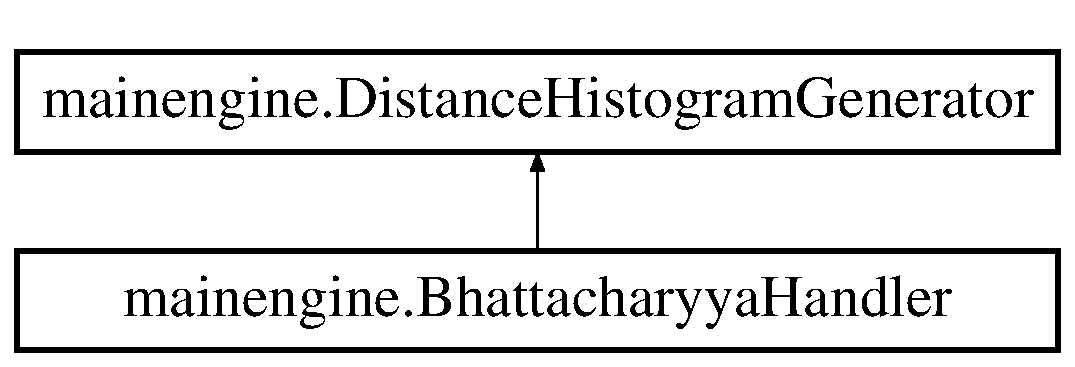
\includegraphics[height=2.000000cm]{classmainengine_1_1_bhattacharyya_handler}
\end{center}
\end{figure}
\subsection*{Public Member Functions}
\begin{DoxyCompactItemize}
\item 
\hyperlink{classmainengine_1_1_bhattacharyya_handler_acadcb8ecddbf08354628cd771746d67c}{Bhattacharyya\+Handler} ()
\item 
Linked\+List$<$ Double $>$ \hyperlink{classmainengine_1_1_bhattacharyya_handler_aaf0d9ca0ecc056d53a2f6f42f41e0b99}{generate\+Distance\+Array} (Linked\+List$<$ Mat $>$ hist\+Collection)
\end{DoxyCompactItemize}


\subsection{Detailed Description}


Definition at line 8 of file Bhattacharyya\+Handler.\+java.



\subsection{Constructor \& Destructor Documentation}
\hypertarget{classmainengine_1_1_bhattacharyya_handler_acadcb8ecddbf08354628cd771746d67c}{}\label{classmainengine_1_1_bhattacharyya_handler_acadcb8ecddbf08354628cd771746d67c} 
\index{mainengine\+::\+Bhattacharyya\+Handler@{mainengine\+::\+Bhattacharyya\+Handler}!Bhattacharyya\+Handler@{Bhattacharyya\+Handler}}
\index{Bhattacharyya\+Handler@{Bhattacharyya\+Handler}!mainengine\+::\+Bhattacharyya\+Handler@{mainengine\+::\+Bhattacharyya\+Handler}}
\subsubsection{\texorpdfstring{Bhattacharyya\+Handler()}{BhattacharyyaHandler()}}
{\footnotesize\ttfamily mainengine.\+Bhattacharyya\+Handler.\+Bhattacharyya\+Handler (\begin{DoxyParamCaption}{ }\end{DoxyParamCaption})}



Definition at line 12 of file Bhattacharyya\+Handler.\+java.



\subsection{Member Function Documentation}
\hypertarget{classmainengine_1_1_bhattacharyya_handler_aaf0d9ca0ecc056d53a2f6f42f41e0b99}{}\label{classmainengine_1_1_bhattacharyya_handler_aaf0d9ca0ecc056d53a2f6f42f41e0b99} 
\index{mainengine\+::\+Bhattacharyya\+Handler@{mainengine\+::\+Bhattacharyya\+Handler}!generate\+Distance\+Array@{generate\+Distance\+Array}}
\index{generate\+Distance\+Array@{generate\+Distance\+Array}!mainengine\+::\+Bhattacharyya\+Handler@{mainengine\+::\+Bhattacharyya\+Handler}}
\subsubsection{\texorpdfstring{generate\+Distance\+Array()}{generateDistanceArray()}}
{\footnotesize\ttfamily Linked\+List$<$Double$>$ mainengine.\+Bhattacharyya\+Handler.\+generate\+Distance\+Array (\begin{DoxyParamCaption}\item[{Linked\+List$<$ Mat $>$}]{hist\+Collection }\end{DoxyParamCaption})}



Implements \hyperlink{interfacemainengine_1_1_distance_histogram_generator_aae0fe15938495eb06c17644291eb099a}{mainengine.\+Distance\+Histogram\+Generator}.



Definition at line 63 of file Bhattacharyya\+Handler.\+java.



The documentation for this class was generated from the following file\+:\begin{DoxyCompactItemize}
\item 
src/mainengine/\hyperlink{_bhattacharyya_handler_8java}{Bhattacharyya\+Handler.\+java}\end{DoxyCompactItemize}

\hypertarget{interfacemainengine_1_1_distance_histogram_generator}{}\section{mainengine.\+Distance\+Histogram\+Generator Interface Reference}
\label{interfacemainengine_1_1_distance_histogram_generator}\index{mainengine.\+Distance\+Histogram\+Generator@{mainengine.\+Distance\+Histogram\+Generator}}
Inheritance diagram for mainengine.\+Distance\+Histogram\+Generator\+:\begin{figure}[H]
\begin{center}
\leavevmode
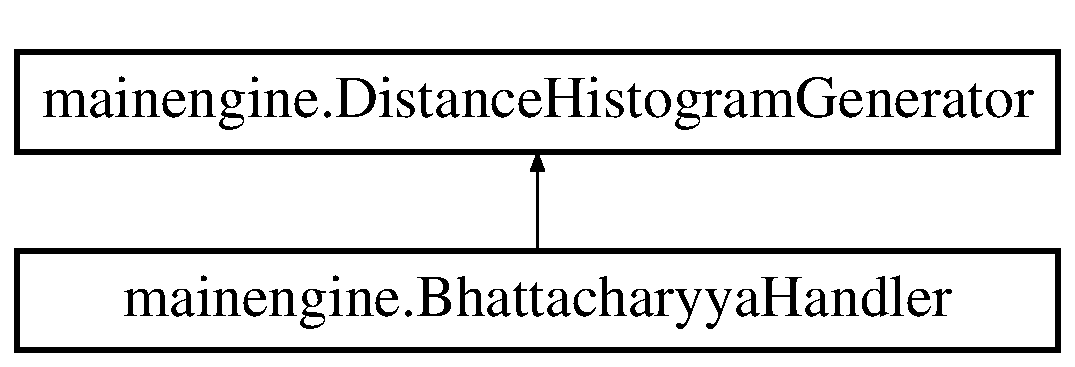
\includegraphics[height=2.000000cm]{interfacemainengine_1_1_distance_histogram_generator}
\end{center}
\end{figure}
\subsection*{Public Member Functions}
\begin{DoxyCompactItemize}
\item 
Linked\+List$<$ Double $>$ \hyperlink{interfacemainengine_1_1_distance_histogram_generator_aae0fe15938495eb06c17644291eb099a}{generate\+Distance\+Array} (Linked\+List$<$ Mat $>$ hist\+Collection)
\end{DoxyCompactItemize}


\subsection{Detailed Description}


Definition at line 9 of file Distance\+Histogram\+Generator.\+java.



\subsection{Member Function Documentation}
\hypertarget{interfacemainengine_1_1_distance_histogram_generator_aae0fe15938495eb06c17644291eb099a}{}\label{interfacemainengine_1_1_distance_histogram_generator_aae0fe15938495eb06c17644291eb099a} 
\index{mainengine\+::\+Distance\+Histogram\+Generator@{mainengine\+::\+Distance\+Histogram\+Generator}!generate\+Distance\+Array@{generate\+Distance\+Array}}
\index{generate\+Distance\+Array@{generate\+Distance\+Array}!mainengine\+::\+Distance\+Histogram\+Generator@{mainengine\+::\+Distance\+Histogram\+Generator}}
\subsubsection{\texorpdfstring{generate\+Distance\+Array()}{generateDistanceArray()}}
{\footnotesize\ttfamily Linked\+List$<$Double$>$ mainengine.\+Distance\+Histogram\+Generator.\+generate\+Distance\+Array (\begin{DoxyParamCaption}\item[{Linked\+List$<$ Mat $>$}]{hist\+Collection }\end{DoxyParamCaption})}



Implemented in \hyperlink{classmainengine_1_1_bhattacharyya_handler_aaf0d9ca0ecc056d53a2f6f42f41e0b99}{mainengine.\+Bhattacharyya\+Handler}.



The documentation for this interface was generated from the following file\+:\begin{DoxyCompactItemize}
\item 
src/mainengine/\hyperlink{_distance_histogram_generator_8java}{Distance\+Histogram\+Generator.\+java}\end{DoxyCompactItemize}

\hypertarget{classmainengine_1_1_histogram_processor}{}\section{mainengine.\+Histogram\+Processor Class Reference}
\label{classmainengine_1_1_histogram_processor}\index{mainengine.\+Histogram\+Processor@{mainengine.\+Histogram\+Processor}}
\subsection*{Public Member Functions}
\begin{DoxyCompactItemize}
\item 
\hyperlink{classmainengine_1_1_histogram_processor_a357b5277d361f75b17473832ef789c3d}{Histogram\+Processor} ()
\item 
Linked\+List$<$ Mat $>$ \hyperlink{classmainengine_1_1_histogram_processor_a5bd85446efa3f4d33a6dd02e34bafce6}{calculate\+Histo\+Of\+Hue\+Video} (Linked\+List$<$ Mat $>$ images)
\item 
void \hyperlink{classmainengine_1_1_histogram_processor_adff19084e721e59757acca5b259f8161}{draw\+Histogram} (Mat histogramH, String name, int width, int height)
\end{DoxyCompactItemize}


\subsection{Detailed Description}


Definition at line 16 of file Histogram\+Processor.\+java.



\subsection{Constructor \& Destructor Documentation}
\hypertarget{classmainengine_1_1_histogram_processor_a357b5277d361f75b17473832ef789c3d}{}\label{classmainengine_1_1_histogram_processor_a357b5277d361f75b17473832ef789c3d} 
\index{mainengine\+::\+Histogram\+Processor@{mainengine\+::\+Histogram\+Processor}!Histogram\+Processor@{Histogram\+Processor}}
\index{Histogram\+Processor@{Histogram\+Processor}!mainengine\+::\+Histogram\+Processor@{mainengine\+::\+Histogram\+Processor}}
\subsubsection{\texorpdfstring{Histogram\+Processor()}{HistogramProcessor()}}
{\footnotesize\ttfamily mainengine.\+Histogram\+Processor.\+Histogram\+Processor (\begin{DoxyParamCaption}{ }\end{DoxyParamCaption})}



Definition at line 21 of file Histogram\+Processor.\+java.



\subsection{Member Function Documentation}
\hypertarget{classmainengine_1_1_histogram_processor_a5bd85446efa3f4d33a6dd02e34bafce6}{}\label{classmainengine_1_1_histogram_processor_a5bd85446efa3f4d33a6dd02e34bafce6} 
\index{mainengine\+::\+Histogram\+Processor@{mainengine\+::\+Histogram\+Processor}!calculate\+Histo\+Of\+Hue\+Video@{calculate\+Histo\+Of\+Hue\+Video}}
\index{calculate\+Histo\+Of\+Hue\+Video@{calculate\+Histo\+Of\+Hue\+Video}!mainengine\+::\+Histogram\+Processor@{mainengine\+::\+Histogram\+Processor}}
\subsubsection{\texorpdfstring{calculate\+Histo\+Of\+Hue\+Video()}{calculateHistoOfHueVideo()}}
{\footnotesize\ttfamily Linked\+List$<$Mat$>$ mainengine.\+Histogram\+Processor.\+calculate\+Histo\+Of\+Hue\+Video (\begin{DoxyParamCaption}\item[{Linked\+List$<$ Mat $>$}]{images }\end{DoxyParamCaption})}



Definition at line 31 of file Histogram\+Processor.\+java.

\hypertarget{classmainengine_1_1_histogram_processor_adff19084e721e59757acca5b259f8161}{}\label{classmainengine_1_1_histogram_processor_adff19084e721e59757acca5b259f8161} 
\index{mainengine\+::\+Histogram\+Processor@{mainengine\+::\+Histogram\+Processor}!draw\+Histogram@{draw\+Histogram}}
\index{draw\+Histogram@{draw\+Histogram}!mainengine\+::\+Histogram\+Processor@{mainengine\+::\+Histogram\+Processor}}
\subsubsection{\texorpdfstring{draw\+Histogram()}{drawHistogram()}}
{\footnotesize\ttfamily void mainengine.\+Histogram\+Processor.\+draw\+Histogram (\begin{DoxyParamCaption}\item[{Mat}]{histogramH,  }\item[{String}]{name,  }\item[{int}]{width,  }\item[{int}]{height }\end{DoxyParamCaption})}



Definition at line 77 of file Histogram\+Processor.\+java.



The documentation for this class was generated from the following file\+:\begin{DoxyCompactItemize}
\item 
src/mainengine/\hyperlink{_histogram_processor_8java}{Histogram\+Processor.\+java}\end{DoxyCompactItemize}

\hypertarget{classmainengine_1_1_main_processor}{}\section{mainengine.\+Main\+Processor Class Reference}
\label{classmainengine_1_1_main_processor}\index{mainengine.\+Main\+Processor@{mainengine.\+Main\+Processor}}
\subsection*{Public Member Functions}
\begin{DoxyCompactItemize}
\item 
\hyperlink{classmainengine_1_1_main_processor_a8a2da887501877affcb70982982c5d1d}{Main\+Processor} ()
\item 
void \hyperlink{classmainengine_1_1_main_processor_aee5d6816bb2dc27ea02ef5f5c4cd3355}{set\+Environment} ()
\item 
Boolean \hyperlink{classmainengine_1_1_main_processor_a270957b142cfc8aa430636545b29679f}{start\+Mainflow} (String video\+Route)
\end{DoxyCompactItemize}


\subsection{Detailed Description}


Definition at line 11 of file Main\+Processor.\+java.



\subsection{Constructor \& Destructor Documentation}
\hypertarget{classmainengine_1_1_main_processor_a8a2da887501877affcb70982982c5d1d}{}\label{classmainengine_1_1_main_processor_a8a2da887501877affcb70982982c5d1d} 
\index{mainengine\+::\+Main\+Processor@{mainengine\+::\+Main\+Processor}!Main\+Processor@{Main\+Processor}}
\index{Main\+Processor@{Main\+Processor}!mainengine\+::\+Main\+Processor@{mainengine\+::\+Main\+Processor}}
\subsubsection{\texorpdfstring{Main\+Processor()}{MainProcessor()}}
{\footnotesize\ttfamily mainengine.\+Main\+Processor.\+Main\+Processor (\begin{DoxyParamCaption}{ }\end{DoxyParamCaption})}



Definition at line 27 of file Main\+Processor.\+java.



\subsection{Member Function Documentation}
\hypertarget{classmainengine_1_1_main_processor_aee5d6816bb2dc27ea02ef5f5c4cd3355}{}\label{classmainengine_1_1_main_processor_aee5d6816bb2dc27ea02ef5f5c4cd3355} 
\index{mainengine\+::\+Main\+Processor@{mainengine\+::\+Main\+Processor}!set\+Environment@{set\+Environment}}
\index{set\+Environment@{set\+Environment}!mainengine\+::\+Main\+Processor@{mainengine\+::\+Main\+Processor}}
\subsubsection{\texorpdfstring{set\+Environment()}{setEnvironment()}}
{\footnotesize\ttfamily void mainengine.\+Main\+Processor.\+set\+Environment (\begin{DoxyParamCaption}{ }\end{DoxyParamCaption})}



Definition at line 31 of file Main\+Processor.\+java.

\hypertarget{classmainengine_1_1_main_processor_a270957b142cfc8aa430636545b29679f}{}\label{classmainengine_1_1_main_processor_a270957b142cfc8aa430636545b29679f} 
\index{mainengine\+::\+Main\+Processor@{mainengine\+::\+Main\+Processor}!start\+Mainflow@{start\+Mainflow}}
\index{start\+Mainflow@{start\+Mainflow}!mainengine\+::\+Main\+Processor@{mainengine\+::\+Main\+Processor}}
\subsubsection{\texorpdfstring{start\+Mainflow()}{startMainflow()}}
{\footnotesize\ttfamily Boolean mainengine.\+Main\+Processor.\+start\+Mainflow (\begin{DoxyParamCaption}\item[{String}]{video\+Route }\end{DoxyParamCaption})}

Function that receives the local route to a video file and validates if it contains a video.


\begin{DoxyParams}{Parameters}
{\em video\+Route} & Route to a local video file. \\
\hline
\end{DoxyParams}
\begin{DoxyReturn}{Returns}
Boolean saying if a route to a video file is valid. 
\end{DoxyReturn}


Definition at line 44 of file Main\+Processor.\+java.



The documentation for this class was generated from the following file\+:\begin{DoxyCompactItemize}
\item 
src/mainengine/\hyperlink{_main_processor_8java}{Main\+Processor.\+java}\end{DoxyCompactItemize}

\hypertarget{classserver_1_1_my_web_socket_handler}{}\section{server.\+My\+Web\+Socket\+Handler Class Reference}
\label{classserver_1_1_my_web_socket_handler}\index{server.\+My\+Web\+Socket\+Handler@{server.\+My\+Web\+Socket\+Handler}}
\subsection*{Public Member Functions}
\begin{DoxyCompactItemize}
\item 
void \hyperlink{classserver_1_1_my_web_socket_handler_a5e3913fe552aa08c6e80f79ff3d3fc01}{on\+Close} (int status\+Code, String reason)
\item 
void \hyperlink{classserver_1_1_my_web_socket_handler_ab232bcea3e901fe731840e6de8c1544b}{on\+Error} (Throwable thrown)
\item 
void \hyperlink{classserver_1_1_my_web_socket_handler_aeff7fa4f5f0e42526174016f05101ba4}{on\+Connect} (Session session)
\item 
void \hyperlink{classserver_1_1_my_web_socket_handler_ad10604d60be64a1af67abba528769fd7}{on\+Message} (String message)
\end{DoxyCompactItemize}


\subsection{Detailed Description}


Definition at line 15 of file My\+Web\+Socket\+Handler.\+java.



\subsection{Member Function Documentation}
\hypertarget{classserver_1_1_my_web_socket_handler_a5e3913fe552aa08c6e80f79ff3d3fc01}{}\label{classserver_1_1_my_web_socket_handler_a5e3913fe552aa08c6e80f79ff3d3fc01} 
\index{server\+::\+My\+Web\+Socket\+Handler@{server\+::\+My\+Web\+Socket\+Handler}!on\+Close@{on\+Close}}
\index{on\+Close@{on\+Close}!server\+::\+My\+Web\+Socket\+Handler@{server\+::\+My\+Web\+Socket\+Handler}}
\subsubsection{\texorpdfstring{on\+Close()}{onClose()}}
{\footnotesize\ttfamily void server.\+My\+Web\+Socket\+Handler.\+on\+Close (\begin{DoxyParamCaption}\item[{int}]{status\+Code,  }\item[{String}]{reason }\end{DoxyParamCaption})}



Definition at line 19 of file My\+Web\+Socket\+Handler.\+java.

\hypertarget{classserver_1_1_my_web_socket_handler_aeff7fa4f5f0e42526174016f05101ba4}{}\label{classserver_1_1_my_web_socket_handler_aeff7fa4f5f0e42526174016f05101ba4} 
\index{server\+::\+My\+Web\+Socket\+Handler@{server\+::\+My\+Web\+Socket\+Handler}!on\+Connect@{on\+Connect}}
\index{on\+Connect@{on\+Connect}!server\+::\+My\+Web\+Socket\+Handler@{server\+::\+My\+Web\+Socket\+Handler}}
\subsubsection{\texorpdfstring{on\+Connect()}{onConnect()}}
{\footnotesize\ttfamily void server.\+My\+Web\+Socket\+Handler.\+on\+Connect (\begin{DoxyParamCaption}\item[{Session}]{session }\end{DoxyParamCaption})}

Function that declares what happens when something connects to the socket. 
\begin{DoxyParams}{Parameters}
{\em session} & Parameter given by the socket class, not given by code. \\
\hline
\end{DoxyParams}


Definition at line 32 of file My\+Web\+Socket\+Handler.\+java.

\hypertarget{classserver_1_1_my_web_socket_handler_ab232bcea3e901fe731840e6de8c1544b}{}\label{classserver_1_1_my_web_socket_handler_ab232bcea3e901fe731840e6de8c1544b} 
\index{server\+::\+My\+Web\+Socket\+Handler@{server\+::\+My\+Web\+Socket\+Handler}!on\+Error@{on\+Error}}
\index{on\+Error@{on\+Error}!server\+::\+My\+Web\+Socket\+Handler@{server\+::\+My\+Web\+Socket\+Handler}}
\subsubsection{\texorpdfstring{on\+Error()}{onError()}}
{\footnotesize\ttfamily void server.\+My\+Web\+Socket\+Handler.\+on\+Error (\begin{DoxyParamCaption}\item[{Throwable}]{thrown }\end{DoxyParamCaption})}



Definition at line 24 of file My\+Web\+Socket\+Handler.\+java.

\hypertarget{classserver_1_1_my_web_socket_handler_ad10604d60be64a1af67abba528769fd7}{}\label{classserver_1_1_my_web_socket_handler_ad10604d60be64a1af67abba528769fd7} 
\index{server\+::\+My\+Web\+Socket\+Handler@{server\+::\+My\+Web\+Socket\+Handler}!on\+Message@{on\+Message}}
\index{on\+Message@{on\+Message}!server\+::\+My\+Web\+Socket\+Handler@{server\+::\+My\+Web\+Socket\+Handler}}
\subsubsection{\texorpdfstring{on\+Message()}{onMessage()}}
{\footnotesize\ttfamily void server.\+My\+Web\+Socket\+Handler.\+on\+Message (\begin{DoxyParamCaption}\item[{String}]{message }\end{DoxyParamCaption})}

Function that declares what to answer to the client whenever the socket receives a message. 
\begin{DoxyParams}{Parameters}
{\em message} & Parameter given by the socket class, not given by code. Contains the message received by the client. \\
\hline
\end{DoxyParams}


Definition at line 46 of file My\+Web\+Socket\+Handler.\+java.



The documentation for this class was generated from the following file\+:\begin{DoxyCompactItemize}
\item 
src/server/\hyperlink{_my_web_socket_handler_8java}{My\+Web\+Socket\+Handler.\+java}\end{DoxyCompactItemize}

\hypertarget{classmainengine_1_1_numerical_data_calculator}{}\section{mainengine.\+Numerical\+Data\+Calculator Class Reference}
\label{classmainengine_1_1_numerical_data_calculator}\index{mainengine.\+Numerical\+Data\+Calculator@{mainengine.\+Numerical\+Data\+Calculator}}
Inheritance diagram for mainengine.\+Numerical\+Data\+Calculator\+:\begin{figure}[H]
\begin{center}
\leavevmode
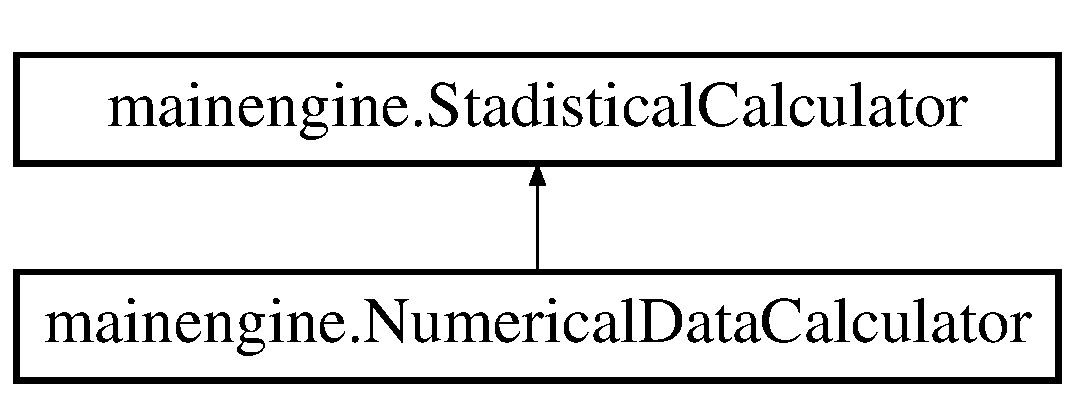
\includegraphics[height=2.000000cm]{classmainengine_1_1_numerical_data_calculator}
\end{center}
\end{figure}
\subsection*{Public Member Functions}
\begin{DoxyCompactItemize}
\item 
\hyperlink{classmainengine_1_1_numerical_data_calculator_aa9166a8e6a28ab6eeab9859c2b7b2701}{Numerical\+Data\+Calculator} ()
\item 
double \hyperlink{classmainengine_1_1_numerical_data_calculator_ac1f0d9cc0a35c84dc092b4c8b4fcd3ed}{calculate\+Average} (Linked\+List$<$ Double $>$ set)
\item 
double \hyperlink{classmainengine_1_1_numerical_data_calculator_ab0ceb7615ed1d5df5b1cae8d47895e7a}{calculate\+Std\+Deviation} (Linked\+List$<$ Double $>$ set)
\end{DoxyCompactItemize}


\subsection{Detailed Description}


Definition at line 5 of file Numerical\+Data\+Calculator.\+java.



\subsection{Constructor \& Destructor Documentation}
\hypertarget{classmainengine_1_1_numerical_data_calculator_aa9166a8e6a28ab6eeab9859c2b7b2701}{}\label{classmainengine_1_1_numerical_data_calculator_aa9166a8e6a28ab6eeab9859c2b7b2701} 
\index{mainengine\+::\+Numerical\+Data\+Calculator@{mainengine\+::\+Numerical\+Data\+Calculator}!Numerical\+Data\+Calculator@{Numerical\+Data\+Calculator}}
\index{Numerical\+Data\+Calculator@{Numerical\+Data\+Calculator}!mainengine\+::\+Numerical\+Data\+Calculator@{mainengine\+::\+Numerical\+Data\+Calculator}}
\subsubsection{\texorpdfstring{Numerical\+Data\+Calculator()}{NumericalDataCalculator()}}
{\footnotesize\ttfamily mainengine.\+Numerical\+Data\+Calculator.\+Numerical\+Data\+Calculator (\begin{DoxyParamCaption}{ }\end{DoxyParamCaption})}



Definition at line 19 of file Numerical\+Data\+Calculator.\+java.



\subsection{Member Function Documentation}
\hypertarget{classmainengine_1_1_numerical_data_calculator_ac1f0d9cc0a35c84dc092b4c8b4fcd3ed}{}\label{classmainengine_1_1_numerical_data_calculator_ac1f0d9cc0a35c84dc092b4c8b4fcd3ed} 
\index{mainengine\+::\+Numerical\+Data\+Calculator@{mainengine\+::\+Numerical\+Data\+Calculator}!calculate\+Average@{calculate\+Average}}
\index{calculate\+Average@{calculate\+Average}!mainengine\+::\+Numerical\+Data\+Calculator@{mainengine\+::\+Numerical\+Data\+Calculator}}
\subsubsection{\texorpdfstring{calculate\+Average()}{calculateAverage()}}
{\footnotesize\ttfamily double mainengine.\+Numerical\+Data\+Calculator.\+calculate\+Average (\begin{DoxyParamCaption}\item[{Linked\+List$<$ Double $>$}]{set }\end{DoxyParamCaption})}



Implements \hyperlink{interfacemainengine_1_1_stadistical_calculator_abf970c09783d3f60e597256a97b936db}{mainengine.\+Stadistical\+Calculator}.



Definition at line 22 of file Numerical\+Data\+Calculator.\+java.

\hypertarget{classmainengine_1_1_numerical_data_calculator_ab0ceb7615ed1d5df5b1cae8d47895e7a}{}\label{classmainengine_1_1_numerical_data_calculator_ab0ceb7615ed1d5df5b1cae8d47895e7a} 
\index{mainengine\+::\+Numerical\+Data\+Calculator@{mainengine\+::\+Numerical\+Data\+Calculator}!calculate\+Std\+Deviation@{calculate\+Std\+Deviation}}
\index{calculate\+Std\+Deviation@{calculate\+Std\+Deviation}!mainengine\+::\+Numerical\+Data\+Calculator@{mainengine\+::\+Numerical\+Data\+Calculator}}
\subsubsection{\texorpdfstring{calculate\+Std\+Deviation()}{calculateStdDeviation()}}
{\footnotesize\ttfamily double mainengine.\+Numerical\+Data\+Calculator.\+calculate\+Std\+Deviation (\begin{DoxyParamCaption}\item[{Linked\+List$<$ Double $>$}]{set }\end{DoxyParamCaption})}



Implements \hyperlink{interfacemainengine_1_1_stadistical_calculator_a48e42fd096a3f1e8a0740355ddc104c3}{mainengine.\+Stadistical\+Calculator}.



Definition at line 32 of file Numerical\+Data\+Calculator.\+java.



The documentation for this class was generated from the following file\+:\begin{DoxyCompactItemize}
\item 
src/mainengine/\hyperlink{_numerical_data_calculator_8java}{Numerical\+Data\+Calculator.\+java}\end{DoxyCompactItemize}

\hypertarget{interfacemainengine_1_1_stadistical_calculator}{}\section{mainengine.\+Stadistical\+Calculator Interface Reference}
\label{interfacemainengine_1_1_stadistical_calculator}\index{mainengine.\+Stadistical\+Calculator@{mainengine.\+Stadistical\+Calculator}}
Inheritance diagram for mainengine.\+Stadistical\+Calculator\+:\begin{figure}[H]
\begin{center}
\leavevmode
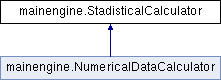
\includegraphics[height=2.000000cm]{interfacemainengine_1_1_stadistical_calculator}
\end{center}
\end{figure}
\subsection*{Public Member Functions}
\begin{DoxyCompactItemize}
\item 
double \hyperlink{interfacemainengine_1_1_stadistical_calculator_abf970c09783d3f60e597256a97b936db}{calculate\+Average} (Linked\+List$<$ Double $>$ set)
\item 
double \hyperlink{interfacemainengine_1_1_stadistical_calculator_a48e42fd096a3f1e8a0740355ddc104c3}{calculate\+Std\+Deviation} (Linked\+List$<$ Double $>$ set)
\end{DoxyCompactItemize}


\subsection{Detailed Description}


Definition at line 5 of file Stadistical\+Calculator.\+java.



\subsection{Member Function Documentation}
\hypertarget{interfacemainengine_1_1_stadistical_calculator_abf970c09783d3f60e597256a97b936db}{}\label{interfacemainengine_1_1_stadistical_calculator_abf970c09783d3f60e597256a97b936db} 
\index{mainengine\+::\+Stadistical\+Calculator@{mainengine\+::\+Stadistical\+Calculator}!calculate\+Average@{calculate\+Average}}
\index{calculate\+Average@{calculate\+Average}!mainengine\+::\+Stadistical\+Calculator@{mainengine\+::\+Stadistical\+Calculator}}
\subsubsection{\texorpdfstring{calculate\+Average()}{calculateAverage()}}
{\footnotesize\ttfamily double mainengine.\+Stadistical\+Calculator.\+calculate\+Average (\begin{DoxyParamCaption}\item[{Linked\+List$<$ Double $>$}]{set }\end{DoxyParamCaption})}



Implemented in \hyperlink{classmainengine_1_1_numerical_data_calculator_ac1f0d9cc0a35c84dc092b4c8b4fcd3ed}{mainengine.\+Numerical\+Data\+Calculator}.

\hypertarget{interfacemainengine_1_1_stadistical_calculator_a48e42fd096a3f1e8a0740355ddc104c3}{}\label{interfacemainengine_1_1_stadistical_calculator_a48e42fd096a3f1e8a0740355ddc104c3} 
\index{mainengine\+::\+Stadistical\+Calculator@{mainengine\+::\+Stadistical\+Calculator}!calculate\+Std\+Deviation@{calculate\+Std\+Deviation}}
\index{calculate\+Std\+Deviation@{calculate\+Std\+Deviation}!mainengine\+::\+Stadistical\+Calculator@{mainengine\+::\+Stadistical\+Calculator}}
\subsubsection{\texorpdfstring{calculate\+Std\+Deviation()}{calculateStdDeviation()}}
{\footnotesize\ttfamily double mainengine.\+Stadistical\+Calculator.\+calculate\+Std\+Deviation (\begin{DoxyParamCaption}\item[{Linked\+List$<$ Double $>$}]{set }\end{DoxyParamCaption})}



Implemented in \hyperlink{classmainengine_1_1_numerical_data_calculator_ab0ceb7615ed1d5df5b1cae8d47895e7a}{mainengine.\+Numerical\+Data\+Calculator}.



The documentation for this interface was generated from the following file\+:\begin{DoxyCompactItemize}
\item 
src/mainengine/\hyperlink{_stadistical_calculator_8java}{Stadistical\+Calculator.\+java}\end{DoxyCompactItemize}

\hypertarget{classunittests_1_1_testjunit0}{}\section{unittests.\+Testjunit0 Class Reference}
\label{classunittests_1_1_testjunit0}\index{unittests.\+Testjunit0@{unittests.\+Testjunit0}}
\subsection*{Public Member Functions}
\begin{DoxyCompactItemize}
\item 
\hyperlink{classunittests_1_1_testjunit0_a51fec7642572da856d10d6f5e6c39df0}{Testjunit0} (String video\+Route, boolean expectedresult)
\item 
void \hyperlink{classunittests_1_1_testjunit0_a520f37a3bb806eb5b0aefa1d88db6d08}{validate\+Complete\+Process} ()
\end{DoxyCompactItemize}
\subsection*{Static Public Member Functions}
\begin{DoxyCompactItemize}
\item 
.Parameters static Collection \hyperlink{classunittests_1_1_testjunit0_a0958eee4a9d97a07f0d5fded1d80551a}{parameters\+To\+Test} ()
\end{DoxyCompactItemize}


\subsection{Detailed Description}


Definition at line 24 of file Testjunit0.\+java.



\subsection{Constructor \& Destructor Documentation}
\hypertarget{classunittests_1_1_testjunit0_a51fec7642572da856d10d6f5e6c39df0}{}\label{classunittests_1_1_testjunit0_a51fec7642572da856d10d6f5e6c39df0} 
\index{unittests\+::\+Testjunit0@{unittests\+::\+Testjunit0}!Testjunit0@{Testjunit0}}
\index{Testjunit0@{Testjunit0}!unittests\+::\+Testjunit0@{unittests\+::\+Testjunit0}}
\subsubsection{\texorpdfstring{Testjunit0()}{Testjunit0()}}
{\footnotesize\ttfamily unittests.\+Testjunit0.\+Testjunit0 (\begin{DoxyParamCaption}\item[{String}]{video\+Route,  }\item[{boolean}]{expectedresult }\end{DoxyParamCaption})}



Definition at line 40 of file Testjunit0.\+java.



\subsection{Member Function Documentation}
\hypertarget{classunittests_1_1_testjunit0_a0958eee4a9d97a07f0d5fded1d80551a}{}\label{classunittests_1_1_testjunit0_a0958eee4a9d97a07f0d5fded1d80551a} 
\index{unittests\+::\+Testjunit0@{unittests\+::\+Testjunit0}!parameters\+To\+Test@{parameters\+To\+Test}}
\index{parameters\+To\+Test@{parameters\+To\+Test}!unittests\+::\+Testjunit0@{unittests\+::\+Testjunit0}}
\subsubsection{\texorpdfstring{parameters\+To\+Test()}{parametersToTest()}}
{\footnotesize\ttfamily .Parameters static Collection unittests.\+Testjunit0.\+parameters\+To\+Test (\begin{DoxyParamCaption}{ }\end{DoxyParamCaption})\hspace{0.3cm}{\ttfamily [static]}}



Definition at line 46 of file Testjunit0.\+java.

\hypertarget{classunittests_1_1_testjunit0_a520f37a3bb806eb5b0aefa1d88db6d08}{}\label{classunittests_1_1_testjunit0_a520f37a3bb806eb5b0aefa1d88db6d08} 
\index{unittests\+::\+Testjunit0@{unittests\+::\+Testjunit0}!validate\+Complete\+Process@{validate\+Complete\+Process}}
\index{validate\+Complete\+Process@{validate\+Complete\+Process}!unittests\+::\+Testjunit0@{unittests\+::\+Testjunit0}}
\subsubsection{\texorpdfstring{validate\+Complete\+Process()}{validateCompleteProcess()}}
{\footnotesize\ttfamily void unittests.\+Testjunit0.\+validate\+Complete\+Process (\begin{DoxyParamCaption}{ }\end{DoxyParamCaption})}



Definition at line 55 of file Testjunit0.\+java.



The documentation for this class was generated from the following file\+:\begin{DoxyCompactItemize}
\item 
src/unittests/\hyperlink{_testjunit0_8java}{Testjunit0.\+java}\end{DoxyCompactItemize}

\hypertarget{classunittests_1_1_testjunit1}{}\section{unittests.\+Testjunit1 Class Reference}
\label{classunittests_1_1_testjunit1}\index{unittests.\+Testjunit1@{unittests.\+Testjunit1}}
\subsection*{Public Member Functions}
\begin{DoxyCompactItemize}
\item 
\hyperlink{classunittests_1_1_testjunit1_ab9b56c0754e0cac4b65c466b21372015}{Testjunit1} (Linked\+List$<$ Double $>$ parameter, double expected\+Result\+Std\+Dev, double expected\+Result\+Avg)
\item 
void \hyperlink{classunittests_1_1_testjunit1_a0d8d17ba74c353e33339cd9abdb9a85b}{test\+Std\+Dev\+Calc} ()
\item 
void \hyperlink{classunittests_1_1_testjunit1_a622923ae23252a93c4926cf21952f3b0}{test\+Avg\+Calc} ()
\end{DoxyCompactItemize}
\subsection*{Static Public Member Functions}
\begin{DoxyCompactItemize}
\item 
.Parameters static Collection \hyperlink{classunittests_1_1_testjunit1_aabef7b871ed456bd558ac96cc1d775e2}{parameters\+To\+Test} ()
\end{DoxyCompactItemize}


\subsection{Detailed Description}


Definition at line 21 of file Testjunit1.\+java.



\subsection{Constructor \& Destructor Documentation}
\hypertarget{classunittests_1_1_testjunit1_ab9b56c0754e0cac4b65c466b21372015}{}\label{classunittests_1_1_testjunit1_ab9b56c0754e0cac4b65c466b21372015} 
\index{unittests\+::\+Testjunit1@{unittests\+::\+Testjunit1}!Testjunit1@{Testjunit1}}
\index{Testjunit1@{Testjunit1}!unittests\+::\+Testjunit1@{unittests\+::\+Testjunit1}}
\subsubsection{\texorpdfstring{Testjunit1()}{Testjunit1()}}
{\footnotesize\ttfamily unittests.\+Testjunit1.\+Testjunit1 (\begin{DoxyParamCaption}\item[{Linked\+List$<$ Double $>$}]{parameter,  }\item[{double}]{expected\+Result\+Std\+Dev,  }\item[{double}]{expected\+Result\+Avg }\end{DoxyParamCaption})}



Definition at line 37 of file Testjunit1.\+java.



\subsection{Member Function Documentation}
\hypertarget{classunittests_1_1_testjunit1_aabef7b871ed456bd558ac96cc1d775e2}{}\label{classunittests_1_1_testjunit1_aabef7b871ed456bd558ac96cc1d775e2} 
\index{unittests\+::\+Testjunit1@{unittests\+::\+Testjunit1}!parameters\+To\+Test@{parameters\+To\+Test}}
\index{parameters\+To\+Test@{parameters\+To\+Test}!unittests\+::\+Testjunit1@{unittests\+::\+Testjunit1}}
\subsubsection{\texorpdfstring{parameters\+To\+Test()}{parametersToTest()}}
{\footnotesize\ttfamily .Parameters static Collection unittests.\+Testjunit1.\+parameters\+To\+Test (\begin{DoxyParamCaption}{ }\end{DoxyParamCaption})\hspace{0.3cm}{\ttfamily [static]}}



Definition at line 46 of file Testjunit1.\+java.

\hypertarget{classunittests_1_1_testjunit1_a622923ae23252a93c4926cf21952f3b0}{}\label{classunittests_1_1_testjunit1_a622923ae23252a93c4926cf21952f3b0} 
\index{unittests\+::\+Testjunit1@{unittests\+::\+Testjunit1}!test\+Avg\+Calc@{test\+Avg\+Calc}}
\index{test\+Avg\+Calc@{test\+Avg\+Calc}!unittests\+::\+Testjunit1@{unittests\+::\+Testjunit1}}
\subsubsection{\texorpdfstring{test\+Avg\+Calc()}{testAvgCalc()}}
{\footnotesize\ttfamily void unittests.\+Testjunit1.\+test\+Avg\+Calc (\begin{DoxyParamCaption}{ }\end{DoxyParamCaption})}



Definition at line 79 of file Testjunit1.\+java.

\hypertarget{classunittests_1_1_testjunit1_a0d8d17ba74c353e33339cd9abdb9a85b}{}\label{classunittests_1_1_testjunit1_a0d8d17ba74c353e33339cd9abdb9a85b} 
\index{unittests\+::\+Testjunit1@{unittests\+::\+Testjunit1}!test\+Std\+Dev\+Calc@{test\+Std\+Dev\+Calc}}
\index{test\+Std\+Dev\+Calc@{test\+Std\+Dev\+Calc}!unittests\+::\+Testjunit1@{unittests\+::\+Testjunit1}}
\subsubsection{\texorpdfstring{test\+Std\+Dev\+Calc()}{testStdDevCalc()}}
{\footnotesize\ttfamily void unittests.\+Testjunit1.\+test\+Std\+Dev\+Calc (\begin{DoxyParamCaption}{ }\end{DoxyParamCaption})}



Definition at line 72 of file Testjunit1.\+java.



The documentation for this class was generated from the following file\+:\begin{DoxyCompactItemize}
\item 
src/unittests/\hyperlink{_testjunit1_8java}{Testjunit1.\+java}\end{DoxyCompactItemize}

\hypertarget{classunittests_1_1_test_j_unit_classes}{}\section{unittests.\+Test\+J\+Unit\+Classes Class Reference}
\label{classunittests_1_1_test_j_unit_classes}\index{unittests.\+Test\+J\+Unit\+Classes@{unittests.\+Test\+J\+Unit\+Classes}}


\subsection{Detailed Description}


Definition at line 10 of file Test\+J\+Unit\+Classes.\+java.



The documentation for this class was generated from the following file\+:\begin{DoxyCompactItemize}
\item 
src/unittests/\hyperlink{_test_j_unit_classes_8java}{Test\+J\+Unit\+Classes.\+java}\end{DoxyCompactItemize}

\hypertarget{classunittests_1_1_test_runner}{}\section{unittests.\+Test\+Runner Class Reference}
\label{classunittests_1_1_test_runner}\index{unittests.\+Test\+Runner@{unittests.\+Test\+Runner}}
\subsection*{Static Public Member Functions}
\begin{DoxyCompactItemize}
\item 
static void \hyperlink{classunittests_1_1_test_runner_a841d96bab611e0ceeaf85d3fdabbe7a5}{main} (String\mbox{[}$\,$\mbox{]} args)
\end{DoxyCompactItemize}


\subsection{Detailed Description}


Definition at line 9 of file Test\+Runner.\+java.



\subsection{Member Function Documentation}
\hypertarget{classunittests_1_1_test_runner_a841d96bab611e0ceeaf85d3fdabbe7a5}{}\label{classunittests_1_1_test_runner_a841d96bab611e0ceeaf85d3fdabbe7a5} 
\index{unittests\+::\+Test\+Runner@{unittests\+::\+Test\+Runner}!main@{main}}
\index{main@{main}!unittests\+::\+Test\+Runner@{unittests\+::\+Test\+Runner}}
\subsubsection{\texorpdfstring{main()}{main()}}
{\footnotesize\ttfamily static void unittests.\+Test\+Runner.\+main (\begin{DoxyParamCaption}\item[{String \mbox{[}$\,$\mbox{]}}]{args }\end{DoxyParamCaption})\hspace{0.3cm}{\ttfamily [static]}}



Definition at line 10 of file Test\+Runner.\+java.



The documentation for this class was generated from the following file\+:\begin{DoxyCompactItemize}
\item 
src/unittests/\hyperlink{_test_runner_8java}{Test\+Runner.\+java}\end{DoxyCompactItemize}

\hypertarget{classmainengine_1_1_three_sigma_umbralizator}{}\section{mainengine.\+Three\+Sigma\+Umbralizator Class Reference}
\label{classmainengine_1_1_three_sigma_umbralizator}\index{mainengine.\+Three\+Sigma\+Umbralizator@{mainengine.\+Three\+Sigma\+Umbralizator}}
Inheritance diagram for mainengine.\+Three\+Sigma\+Umbralizator\+:\begin{figure}[H]
\begin{center}
\leavevmode
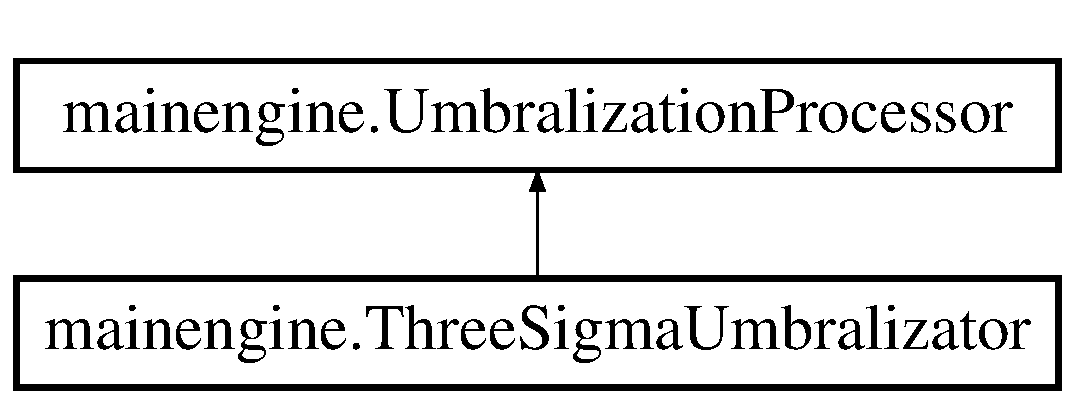
\includegraphics[height=2.000000cm]{classmainengine_1_1_three_sigma_umbralizator}
\end{center}
\end{figure}
\subsection*{Public Member Functions}
\begin{DoxyCompactItemize}
\item 
\hyperlink{classmainengine_1_1_three_sigma_umbralizator_a6ab404b91b56a67cdf00b43ed260af37}{Three\+Sigma\+Umbralizator} ()
\item 
Linked\+List$<$ Boolean $>$ \hyperlink{classmainengine_1_1_three_sigma_umbralizator_a56bfd8fcc856b38e503273e85c0ccf33}{obtain\+Cuts} (Linked\+List$<$ Double $>$ distance\+Hist\+Array)
\end{DoxyCompactItemize}


\subsection{Detailed Description}


Definition at line 6 of file Three\+Sigma\+Umbralizator.\+java.



\subsection{Constructor \& Destructor Documentation}
\hypertarget{classmainengine_1_1_three_sigma_umbralizator_a6ab404b91b56a67cdf00b43ed260af37}{}\label{classmainengine_1_1_three_sigma_umbralizator_a6ab404b91b56a67cdf00b43ed260af37} 
\index{mainengine\+::\+Three\+Sigma\+Umbralizator@{mainengine\+::\+Three\+Sigma\+Umbralizator}!Three\+Sigma\+Umbralizator@{Three\+Sigma\+Umbralizator}}
\index{Three\+Sigma\+Umbralizator@{Three\+Sigma\+Umbralizator}!mainengine\+::\+Three\+Sigma\+Umbralizator@{mainengine\+::\+Three\+Sigma\+Umbralizator}}
\subsubsection{\texorpdfstring{Three\+Sigma\+Umbralizator()}{ThreeSigmaUmbralizator()}}
{\footnotesize\ttfamily mainengine.\+Three\+Sigma\+Umbralizator.\+Three\+Sigma\+Umbralizator (\begin{DoxyParamCaption}{ }\end{DoxyParamCaption})}



Definition at line 8 of file Three\+Sigma\+Umbralizator.\+java.



\subsection{Member Function Documentation}
\hypertarget{classmainengine_1_1_three_sigma_umbralizator_a56bfd8fcc856b38e503273e85c0ccf33}{}\label{classmainengine_1_1_three_sigma_umbralizator_a56bfd8fcc856b38e503273e85c0ccf33} 
\index{mainengine\+::\+Three\+Sigma\+Umbralizator@{mainengine\+::\+Three\+Sigma\+Umbralizator}!obtain\+Cuts@{obtain\+Cuts}}
\index{obtain\+Cuts@{obtain\+Cuts}!mainengine\+::\+Three\+Sigma\+Umbralizator@{mainengine\+::\+Three\+Sigma\+Umbralizator}}
\subsubsection{\texorpdfstring{obtain\+Cuts()}{obtainCuts()}}
{\footnotesize\ttfamily Linked\+List$<$Boolean$>$ mainengine.\+Three\+Sigma\+Umbralizator.\+obtain\+Cuts (\begin{DoxyParamCaption}\item[{Linked\+List$<$ Double $>$}]{distance\+Hist\+Array }\end{DoxyParamCaption})}



Implements \hyperlink{interfacemainengine_1_1_umbralization_processor_ac96dfbad3a28e5332e2cb95ab8996377}{mainengine.\+Umbralization\+Processor}.



Definition at line 20 of file Three\+Sigma\+Umbralizator.\+java.



The documentation for this class was generated from the following file\+:\begin{DoxyCompactItemize}
\item 
src/mainengine/\hyperlink{_three_sigma_umbralizator_8java}{Three\+Sigma\+Umbralizator.\+java}\end{DoxyCompactItemize}

\hypertarget{interfacemainengine_1_1_umbralization_processor}{}\section{mainengine.\+Umbralization\+Processor Interface Reference}
\label{interfacemainengine_1_1_umbralization_processor}\index{mainengine.\+Umbralization\+Processor@{mainengine.\+Umbralization\+Processor}}
Inheritance diagram for mainengine.\+Umbralization\+Processor\+:\begin{figure}[H]
\begin{center}
\leavevmode
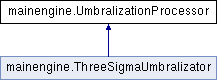
\includegraphics[height=2.000000cm]{interfacemainengine_1_1_umbralization_processor}
\end{center}
\end{figure}
\subsection*{Public Member Functions}
\begin{DoxyCompactItemize}
\item 
Linked\+List$<$ Boolean $>$ \hyperlink{interfacemainengine_1_1_umbralization_processor_ac96dfbad3a28e5332e2cb95ab8996377}{obtain\+Cuts} (Linked\+List$<$ Double $>$ distance\+Hist\+Array)
\end{DoxyCompactItemize}


\subsection{Detailed Description}


Definition at line 7 of file Umbralization\+Processor.\+java.



\subsection{Member Function Documentation}
\hypertarget{interfacemainengine_1_1_umbralization_processor_ac96dfbad3a28e5332e2cb95ab8996377}{}\label{interfacemainengine_1_1_umbralization_processor_ac96dfbad3a28e5332e2cb95ab8996377} 
\index{mainengine\+::\+Umbralization\+Processor@{mainengine\+::\+Umbralization\+Processor}!obtain\+Cuts@{obtain\+Cuts}}
\index{obtain\+Cuts@{obtain\+Cuts}!mainengine\+::\+Umbralization\+Processor@{mainengine\+::\+Umbralization\+Processor}}
\subsubsection{\texorpdfstring{obtain\+Cuts()}{obtainCuts()}}
{\footnotesize\ttfamily Linked\+List$<$Boolean$>$ mainengine.\+Umbralization\+Processor.\+obtain\+Cuts (\begin{DoxyParamCaption}\item[{Linked\+List$<$ Double $>$}]{distance\+Hist\+Array }\end{DoxyParamCaption})}



Implemented in \hyperlink{classmainengine_1_1_three_sigma_umbralizator_a56bfd8fcc856b38e503273e85c0ccf33}{mainengine.\+Three\+Sigma\+Umbralizator}.



The documentation for this interface was generated from the following file\+:\begin{DoxyCompactItemize}
\item 
src/mainengine/\hyperlink{_umbralization_processor_8java}{Umbralization\+Processor.\+java}\end{DoxyCompactItemize}

\hypertarget{classmainengine_1_1_video_segmenter}{}\section{mainengine.\+Video\+Segmenter Class Reference}
\label{classmainengine_1_1_video_segmenter}\index{mainengine.\+Video\+Segmenter@{mainengine.\+Video\+Segmenter}}
\subsection*{Public Member Functions}
\begin{DoxyCompactItemize}
\item 
\hyperlink{classmainengine_1_1_video_segmenter_a2901ca72cf0d9a0e5c3fe7d5a49cbf05}{Video\+Segmenter} ()
\item 
Linked\+List$<$ Mat $>$ \hyperlink{classmainengine_1_1_video_segmenter_ae3e987f60b12c66b3c212646f4a1f9f5}{split\+\_\+video\+\_\+to\+\_\+frames\+\_\+hsv} (String filename)
\item 
void \hyperlink{classmainengine_1_1_video_segmenter_a73f78b10d93a3fe04285a69875b50d01}{create\+Videofromframes} (Linked\+List$<$ Mat $>$ frames, String filenmae,)
\end{DoxyCompactItemize}


\subsection{Detailed Description}


Definition at line 11 of file Video\+Segmenter.\+java.



\subsection{Constructor \& Destructor Documentation}
\hypertarget{classmainengine_1_1_video_segmenter_a2901ca72cf0d9a0e5c3fe7d5a49cbf05}{}\label{classmainengine_1_1_video_segmenter_a2901ca72cf0d9a0e5c3fe7d5a49cbf05} 
\index{mainengine\+::\+Video\+Segmenter@{mainengine\+::\+Video\+Segmenter}!Video\+Segmenter@{Video\+Segmenter}}
\index{Video\+Segmenter@{Video\+Segmenter}!mainengine\+::\+Video\+Segmenter@{mainengine\+::\+Video\+Segmenter}}
\subsubsection{\texorpdfstring{Video\+Segmenter()}{VideoSegmenter()}}
{\footnotesize\ttfamily mainengine.\+Video\+Segmenter.\+Video\+Segmenter (\begin{DoxyParamCaption}{ }\end{DoxyParamCaption})}



Definition at line 42 of file Video\+Segmenter.\+java.



\subsection{Member Function Documentation}
\hypertarget{classmainengine_1_1_video_segmenter_a73f78b10d93a3fe04285a69875b50d01}{}\label{classmainengine_1_1_video_segmenter_a73f78b10d93a3fe04285a69875b50d01} 
\index{mainengine\+::\+Video\+Segmenter@{mainengine\+::\+Video\+Segmenter}!create\+Videofromframes@{create\+Videofromframes}}
\index{create\+Videofromframes@{create\+Videofromframes}!mainengine\+::\+Video\+Segmenter@{mainengine\+::\+Video\+Segmenter}}
\subsubsection{\texorpdfstring{create\+Videofromframes()}{createVideofromframes()}}
{\footnotesize\ttfamily void mainengine.\+Video\+Segmenter.\+create\+Videofromframes (\begin{DoxyParamCaption}\item[{Linked\+List$<$ Mat $>$}]{frames,  }\item[{String}]{filenmae }\end{DoxyParamCaption})}



Definition at line 70 of file Video\+Segmenter.\+java.

\hypertarget{classmainengine_1_1_video_segmenter_ae3e987f60b12c66b3c212646f4a1f9f5}{}\label{classmainengine_1_1_video_segmenter_ae3e987f60b12c66b3c212646f4a1f9f5} 
\index{mainengine\+::\+Video\+Segmenter@{mainengine\+::\+Video\+Segmenter}!split\+\_\+video\+\_\+to\+\_\+frames\+\_\+hsv@{split\+\_\+video\+\_\+to\+\_\+frames\+\_\+hsv}}
\index{split\+\_\+video\+\_\+to\+\_\+frames\+\_\+hsv@{split\+\_\+video\+\_\+to\+\_\+frames\+\_\+hsv}!mainengine\+::\+Video\+Segmenter@{mainengine\+::\+Video\+Segmenter}}
\subsubsection{\texorpdfstring{split\+\_\+video\+\_\+to\+\_\+frames\+\_\+hsv()}{split\_video\_to\_frames\_hsv()}}
{\footnotesize\ttfamily Linked\+List$<$Mat$>$ mainengine.\+Video\+Segmenter.\+split\+\_\+video\+\_\+to\+\_\+frames\+\_\+hsv (\begin{DoxyParamCaption}\item[{String}]{filename }\end{DoxyParamCaption})}

Function that creates H\+SV files from the frames of the video sent.


\begin{DoxyParams}{Parameters}
{\em filename} & String directing to the location of the video file. \\
\hline
\end{DoxyParams}
\begin{DoxyReturn}{Returns}
List of all the H\+SV files made from all the frames of the video. 
\end{DoxyReturn}


Definition at line 52 of file Video\+Segmenter.\+java.



The documentation for this class was generated from the following file\+:\begin{DoxyCompactItemize}
\item 
src/mainengine/\hyperlink{_video_segmenter_8java}{Video\+Segmenter.\+java}\end{DoxyCompactItemize}

\hypertarget{classserver_1_1_web_socket_test}{}\section{server.\+Web\+Socket\+Test Class Reference}
\label{classserver_1_1_web_socket_test}\index{server.\+Web\+Socket\+Test@{server.\+Web\+Socket\+Test}}
\subsection*{Static Public Member Functions}
\begin{DoxyCompactItemize}
\item 
static void \hyperlink{classserver_1_1_web_socket_test_a3e9a6f18d139bb4f32373c7894a8aaf8}{main} (String\mbox{[}$\,$\mbox{]} args)  throws Exception 
\end{DoxyCompactItemize}


\subsection{Detailed Description}


Definition at line 7 of file Web\+Socket\+Test.\+java.



\subsection{Member Function Documentation}
\hypertarget{classserver_1_1_web_socket_test_a3e9a6f18d139bb4f32373c7894a8aaf8}{}\label{classserver_1_1_web_socket_test_a3e9a6f18d139bb4f32373c7894a8aaf8} 
\index{server\+::\+Web\+Socket\+Test@{server\+::\+Web\+Socket\+Test}!main@{main}}
\index{main@{main}!server\+::\+Web\+Socket\+Test@{server\+::\+Web\+Socket\+Test}}
\subsubsection{\texorpdfstring{main()}{main()}}
{\footnotesize\ttfamily static void server.\+Web\+Socket\+Test.\+main (\begin{DoxyParamCaption}\item[{String \mbox{[}$\,$\mbox{]}}]{args }\end{DoxyParamCaption}) throws Exception\hspace{0.3cm}{\ttfamily [static]}}

Main that the server should run to allow the web application to communicate with it. 
\begin{DoxyParams}{Parameters}
{\em args} & Default main arguments. \\
\hline
\end{DoxyParams}

\begin{DoxyExceptions}{Exceptions}
{\em Exception} & Can throw exceptions because of socket connections. \\
\hline
\end{DoxyExceptions}


Definition at line 12 of file Web\+Socket\+Test.\+java.



The documentation for this class was generated from the following file\+:\begin{DoxyCompactItemize}
\item 
src/server/\hyperlink{_web_socket_test_8java}{Web\+Socket\+Test.\+java}\end{DoxyCompactItemize}

\chapter{File Documentation}
\hypertarget{_bhattacharyya_handler_8java}{}\section{src/mainengine/\+Bhattacharyya\+Handler.java File Reference}
\label{_bhattacharyya_handler_8java}\index{src/mainengine/\+Bhattacharyya\+Handler.\+java@{src/mainengine/\+Bhattacharyya\+Handler.\+java}}
\subsection*{Classes}
\begin{DoxyCompactItemize}
\item 
class \hyperlink{classmainengine_1_1_bhattacharyya_handler}{mainengine.\+Bhattacharyya\+Handler}
\end{DoxyCompactItemize}
\subsection*{Packages}
\begin{DoxyCompactItemize}
\item 
package \hyperlink{namespacemainengine}{mainengine}
\end{DoxyCompactItemize}

\hypertarget{_distance_histogram_generator_8java}{}\section{src/mainengine/\+Distance\+Histogram\+Generator.java File Reference}
\label{_distance_histogram_generator_8java}\index{src/mainengine/\+Distance\+Histogram\+Generator.\+java@{src/mainengine/\+Distance\+Histogram\+Generator.\+java}}
\subsection*{Classes}
\begin{DoxyCompactItemize}
\item 
interface \hyperlink{interfacemainengine_1_1_distance_histogram_generator}{mainengine.\+Distance\+Histogram\+Generator}
\end{DoxyCompactItemize}
\subsection*{Packages}
\begin{DoxyCompactItemize}
\item 
package \hyperlink{namespacemainengine}{mainengine}
\end{DoxyCompactItemize}

\hypertarget{_histogram_processor_8java}{}\section{src/mainengine/\+Histogram\+Processor.java File Reference}
\label{_histogram_processor_8java}\index{src/mainengine/\+Histogram\+Processor.\+java@{src/mainengine/\+Histogram\+Processor.\+java}}
\subsection*{Classes}
\begin{DoxyCompactItemize}
\item 
class \hyperlink{classmainengine_1_1_histogram_processor}{mainengine.\+Histogram\+Processor}
\end{DoxyCompactItemize}
\subsection*{Packages}
\begin{DoxyCompactItemize}
\item 
package \hyperlink{namespacemainengine}{mainengine}
\end{DoxyCompactItemize}

\hypertarget{_main_processor_8java}{}\section{src/mainengine/\+Main\+Processor.java File Reference}
\label{_main_processor_8java}\index{src/mainengine/\+Main\+Processor.\+java@{src/mainengine/\+Main\+Processor.\+java}}
\subsection*{Classes}
\begin{DoxyCompactItemize}
\item 
class \hyperlink{classmainengine_1_1_main_processor}{mainengine.\+Main\+Processor}
\end{DoxyCompactItemize}
\subsection*{Packages}
\begin{DoxyCompactItemize}
\item 
package \hyperlink{namespacemainengine}{mainengine}
\end{DoxyCompactItemize}

\hypertarget{_numerical_data_calculator_8java}{}\section{src/mainengine/\+Numerical\+Data\+Calculator.java File Reference}
\label{_numerical_data_calculator_8java}\index{src/mainengine/\+Numerical\+Data\+Calculator.\+java@{src/mainengine/\+Numerical\+Data\+Calculator.\+java}}
\subsection*{Classes}
\begin{DoxyCompactItemize}
\item 
class \hyperlink{classmainengine_1_1_numerical_data_calculator}{mainengine.\+Numerical\+Data\+Calculator}
\end{DoxyCompactItemize}
\subsection*{Packages}
\begin{DoxyCompactItemize}
\item 
package \hyperlink{namespacemainengine}{mainengine}
\end{DoxyCompactItemize}

\hypertarget{_stadistical_calculator_8java}{}\section{src/mainengine/\+Stadistical\+Calculator.java File Reference}
\label{_stadistical_calculator_8java}\index{src/mainengine/\+Stadistical\+Calculator.\+java@{src/mainengine/\+Stadistical\+Calculator.\+java}}
\subsection*{Classes}
\begin{DoxyCompactItemize}
\item 
interface \hyperlink{interfacemainengine_1_1_stadistical_calculator}{mainengine.\+Stadistical\+Calculator}
\end{DoxyCompactItemize}
\subsection*{Packages}
\begin{DoxyCompactItemize}
\item 
package \hyperlink{namespacemainengine}{mainengine}
\end{DoxyCompactItemize}

\hypertarget{_three_sigma_umbralizator_8java}{}\section{src/mainengine/\+Three\+Sigma\+Umbralizator.java File Reference}
\label{_three_sigma_umbralizator_8java}\index{src/mainengine/\+Three\+Sigma\+Umbralizator.\+java@{src/mainengine/\+Three\+Sigma\+Umbralizator.\+java}}
\subsection*{Classes}
\begin{DoxyCompactItemize}
\item 
class \hyperlink{classmainengine_1_1_three_sigma_umbralizator}{mainengine.\+Three\+Sigma\+Umbralizator}
\end{DoxyCompactItemize}
\subsection*{Packages}
\begin{DoxyCompactItemize}
\item 
package \hyperlink{namespacemainengine}{mainengine}
\end{DoxyCompactItemize}

\hypertarget{_umbralization_processor_8java}{}\section{src/mainengine/\+Umbralization\+Processor.java File Reference}
\label{_umbralization_processor_8java}\index{src/mainengine/\+Umbralization\+Processor.\+java@{src/mainengine/\+Umbralization\+Processor.\+java}}
\subsection*{Classes}
\begin{DoxyCompactItemize}
\item 
interface \hyperlink{interfacemainengine_1_1_umbralization_processor}{mainengine.\+Umbralization\+Processor}
\end{DoxyCompactItemize}
\subsection*{Packages}
\begin{DoxyCompactItemize}
\item 
package \hyperlink{namespacemainengine}{mainengine}
\end{DoxyCompactItemize}

\hypertarget{_video_segmenter_8java}{}\section{src/mainengine/\+Video\+Segmenter.java File Reference}
\label{_video_segmenter_8java}\index{src/mainengine/\+Video\+Segmenter.\+java@{src/mainengine/\+Video\+Segmenter.\+java}}
\subsection*{Classes}
\begin{DoxyCompactItemize}
\item 
class \hyperlink{classmainengine_1_1_video_segmenter}{mainengine.\+Video\+Segmenter}
\end{DoxyCompactItemize}
\subsection*{Packages}
\begin{DoxyCompactItemize}
\item 
package \hyperlink{namespacemainengine}{mainengine}
\end{DoxyCompactItemize}

\hypertarget{_my_web_socket_handler_8java}{}\section{src/server/\+My\+Web\+Socket\+Handler.java File Reference}
\label{_my_web_socket_handler_8java}\index{src/server/\+My\+Web\+Socket\+Handler.\+java@{src/server/\+My\+Web\+Socket\+Handler.\+java}}
\subsection*{Classes}
\begin{DoxyCompactItemize}
\item 
class \hyperlink{classserver_1_1_my_web_socket_handler}{server.\+My\+Web\+Socket\+Handler}
\end{DoxyCompactItemize}
\subsection*{Packages}
\begin{DoxyCompactItemize}
\item 
package \hyperlink{namespaceserver}{server}
\end{DoxyCompactItemize}

\hypertarget{_web_socket_test_8java}{}\section{src/server/\+Web\+Socket\+Test.java File Reference}
\label{_web_socket_test_8java}\index{src/server/\+Web\+Socket\+Test.\+java@{src/server/\+Web\+Socket\+Test.\+java}}
\subsection*{Classes}
\begin{DoxyCompactItemize}
\item 
class \hyperlink{classserver_1_1_web_socket_test}{server.\+Web\+Socket\+Test}
\end{DoxyCompactItemize}
\subsection*{Packages}
\begin{DoxyCompactItemize}
\item 
package \hyperlink{namespaceserver}{server}
\end{DoxyCompactItemize}

\hypertarget{_testjunit0_8java}{}\section{src/unittests/\+Testjunit0.java File Reference}
\label{_testjunit0_8java}\index{src/unittests/\+Testjunit0.\+java@{src/unittests/\+Testjunit0.\+java}}
\subsection*{Classes}
\begin{DoxyCompactItemize}
\item 
class \hyperlink{classunittests_1_1_testjunit0}{unittests.\+Testjunit0}
\end{DoxyCompactItemize}
\subsection*{Packages}
\begin{DoxyCompactItemize}
\item 
package \hyperlink{namespaceunittests}{unittests}
\end{DoxyCompactItemize}

\hypertarget{_testjunit1_8java}{}\section{src/unittests/\+Testjunit1.java File Reference}
\label{_testjunit1_8java}\index{src/unittests/\+Testjunit1.\+java@{src/unittests/\+Testjunit1.\+java}}
\subsection*{Classes}
\begin{DoxyCompactItemize}
\item 
class \hyperlink{classunittests_1_1_testjunit1}{unittests.\+Testjunit1}
\end{DoxyCompactItemize}
\subsection*{Packages}
\begin{DoxyCompactItemize}
\item 
package \hyperlink{namespaceunittests}{unittests}
\end{DoxyCompactItemize}

\hypertarget{_test_j_unit_classes_8java}{}\section{src/unittests/\+Test\+J\+Unit\+Classes.java File Reference}
\label{_test_j_unit_classes_8java}\index{src/unittests/\+Test\+J\+Unit\+Classes.\+java@{src/unittests/\+Test\+J\+Unit\+Classes.\+java}}
\subsection*{Classes}
\begin{DoxyCompactItemize}
\item 
class \hyperlink{classunittests_1_1_test_j_unit_classes}{unittests.\+Test\+J\+Unit\+Classes}
\end{DoxyCompactItemize}
\subsection*{Packages}
\begin{DoxyCompactItemize}
\item 
package \hyperlink{namespaceunittests}{unittests}
\end{DoxyCompactItemize}

\hypertarget{_test_runner_8java}{}\section{src/unittests/\+Test\+Runner.java File Reference}
\label{_test_runner_8java}\index{src/unittests/\+Test\+Runner.\+java@{src/unittests/\+Test\+Runner.\+java}}
\subsection*{Classes}
\begin{DoxyCompactItemize}
\item 
class \hyperlink{classunittests_1_1_test_runner}{unittests.\+Test\+Runner}
\end{DoxyCompactItemize}
\subsection*{Packages}
\begin{DoxyCompactItemize}
\item 
package \hyperlink{namespaceunittests}{unittests}
\end{DoxyCompactItemize}

%--- End generated contents ---

% Index
\backmatter
\newpage
\phantomsection
\clearemptydoublepage
\addcontentsline{toc}{chapter}{Index}
\printindex

\end{document}
